\chapter{Exemplu de utilizare: Smart Home}
\label{chapter:studiuCaz}

Pentru a demonstra fiabilitatea platformei, acest capitol propune o soluţie pentru problema automatizării unei case. O asemenea soluţie ieftină şi uşor de implementat lipseşte încă de pe piaţă, sistemele profesionale fiind foarte scumpe, iar cele open-source sunt greu de instalat şi configurat.

Urmărim deci rezolvarea automatizării unei case cu un dormitor şi o sufragerie, în care au fost instalate următoarele dispozitive:
\begin{itemize}
	\item Reţea de senzori inteligenţi, distribuiţi în toate camerele, capabili să ofere informaţii cu privire la numărul de oameni din casă.
	\item Sistem de iluminare inteligent, controlabil de la distanţă.
	\item Un dispozitiv automat de închidere a uşii de la intrare.
\end{itemize}
Automatizarea funcţionează astfel:
\begin{itemize}
	\item Atunci când nu mai există oameni în casă, uşa trebuie încuiată;
	\item La un minut după de camera este liberă lumina din acea cameră este stinsă;
	\item Dacă toţi oamenii se află în dormitor, uşa se încuie automat la ora 00:00.
\end{itemize}

Au fost create următoarele blocuri de intrare, pentru fiecare dispozitiv:
\begin{itemize}
	\item \textbf{Prezenţă Sufragerie}: indică dacă exista persoane in sufragerie. Are un singur canal pe care trimite date de tip întreg despre numărul de oameni din cameră.
	\item \textbf{Prezenţă Dormitor}: senzorul din dormitor, analog cu Prezenţă Sufragerie.
\end{itemize}
\begin{figure}[H]
	\centering
	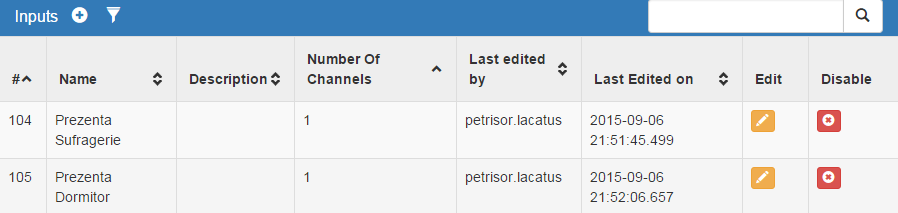
\includegraphics[width=1.1\textwidth, center]{utilizare/inputs}
	\captionsetup{justification=centering}
	\caption{Intrările in aplicaţie}
	\label{fig:inputs}
\end{figure}

Următoarele diagrame au fost implementate:
\begin{itemize}
	\item \textbf{Închidere uşă noaptea}: Comandă închiderea uşii după ora 00:00 dacă toţi oamenii sunt în dormitor;
	\item \textbf{Securizare casa}:  Comandă închiderea uşii când senzorii de prezenţă indică faptul că nu mai sunt persoane \ref{fig:securizareCasa};
	\item \textbf{Oprire lumina dormitor}:  Comandă oprirea luminii când nu mai e nimeni în dormitor;
	\item \textbf{Oprire lumina sufragerie}: Analog, pentru sufragerie;
\end{itemize}

\begin{figure}[H]
	\centering
	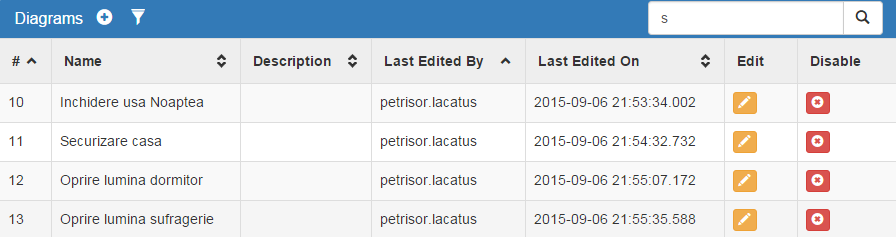
\includegraphics[width=1.1\textwidth, center]{utilizare/diagrams}
	\captionsetup{justification=centering}
	\caption{Diagramele implementate}
	\label{fig:diagrams}
\end{figure}
Spre exemplu, în \cref{fig:securizareCasa} este prezentată diagrama care realizează încuierea casei când nu mai exista persoane în interior. Aceasta foloseşte canalele celor doi senzori de prezentă şi trimite valorile acestora către blocul "\textbf{Adder}", care adună toate intrările numerice. Dacă suma acestor intrări este 0, blocul "\textbf{MaiMareCaZero}" va returna valoarea fals, care este citită de dispozitivul de pe uşă ce acţionează mecanismul de închidere. În caz contrar, valoare returnată de blocul \textbf{MaiMareCaZero} este "adevarat", deci mecanismul nu va fi acţionat. Putem astfel vedea cât de uşor este să implementezi o logica complexă folosind diagrame bloc.
\begin{figure}[H]
	\centering
	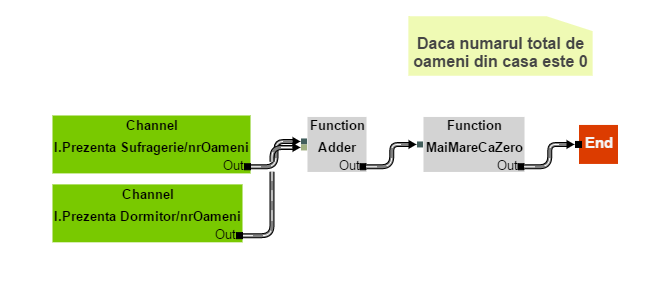
\includegraphics[width=1.1\textwidth, center]{utilizare/securizareCasa}
	\captionsetup{justification=centering}
	\caption{Diagrama pentru securizarea casei}
	\label{fig:securizareCasa}
\end{figure}